
\section{Grundlagen}

Hier erklären was kommt

\subsection{Microservices}

Für den Begriff Microservices existiert keine einheitlich anerkannte Definition. Während Wolff unter Microservices unabhängig, deploybare Module versteht\cite{wolff2018mic_praxis}, spricht Newman von kleinen, autonomen Services, die zusammenarbeiten. Cockcroft verwendet den Begriff Microservice gekoppelt mit einem Architekturbegriff: Eine Microservice Architektur sind gekoppelte Services, welche für einen gewissen Kontextbereich zuständig sind.\cite{irakli2016mic_arc} D.h. jeder Service behandelte gewisse, fachliche Aufgaben und kann genau für diese genutzt werden. Eine Vielzahl von solchen Services bildet dann die gesamte Anwendung. \\

Amudsen schreibt dem Microservice an sich die Eigenschaft zu, dass er unabhängig zu anderen Microservices sein muss, d.h. ein Microservice kann losgelöst von anderen geupdated (deployed) werden. Weiter ist ein Microservice wie schon bei Cockcroft für einen gewissen Aufgabenbereich zuständig. Eine Microservice-Architektur ist ein zusammenschluss von miteinander kommunizierenden Microservices.\cite{irakli2016mic_arc} \\

In \textit{Flexible Software Architecture}\cite{wolff2016mic_architectures} werden Microservices zu den bisherigen noch weitere, teils technische Eigenschaften zugeschrieben: Microservices sind technologisch unabhängig, d.h. eine Microservice Architektur ist beispielsweise nicht an eine bestimmte Programmiersprache oder Datenbank gebunden. Weiter müssen Microservices einen privaten Datenspeicher haben und sie kommunizieren mit anderen Services über das Netzwerk (z.B. über REST). Ebenfalls werden Microservices verwendet, um große Programme in kleine Teile zu unterteilen. Diese kleine Teile lassen sich automatisch bauen und deployen. \\

Basierend auf den folgenden Definitionen wird der Microservice Begriff wie folgt verwendet: Microservices sind
\begin{itemize}
	\item klein in der Größe
	\item kommunizieren mit anderen Services über Netzwerkschnittstellen (z.B. REST) sind unabhängig voneinander deploybar
	\item können unabhängig voneinander entwickelt werden (d.h. Microservice A muss nicht auf B,C,D … warten und/oder umgekehrt)    
	\item eingeschränkt in ihrer Geschäftslogik, d.h. ein Microservice kümmert sich immer um einen speziellen Kontext, der im vorhinein definiert werden muss
	\item dezentral, d.h. sie können auf unterschiedlichsten Plattformen gehosted werden werden automatisch gebaut und deployed
\end{itemize}

Abschließend handelt es sich um eine Microservice-Architektur, wenn viele Microservices nach Definition verwendet werden. 

\begin{figure}[ht]
	\centering
	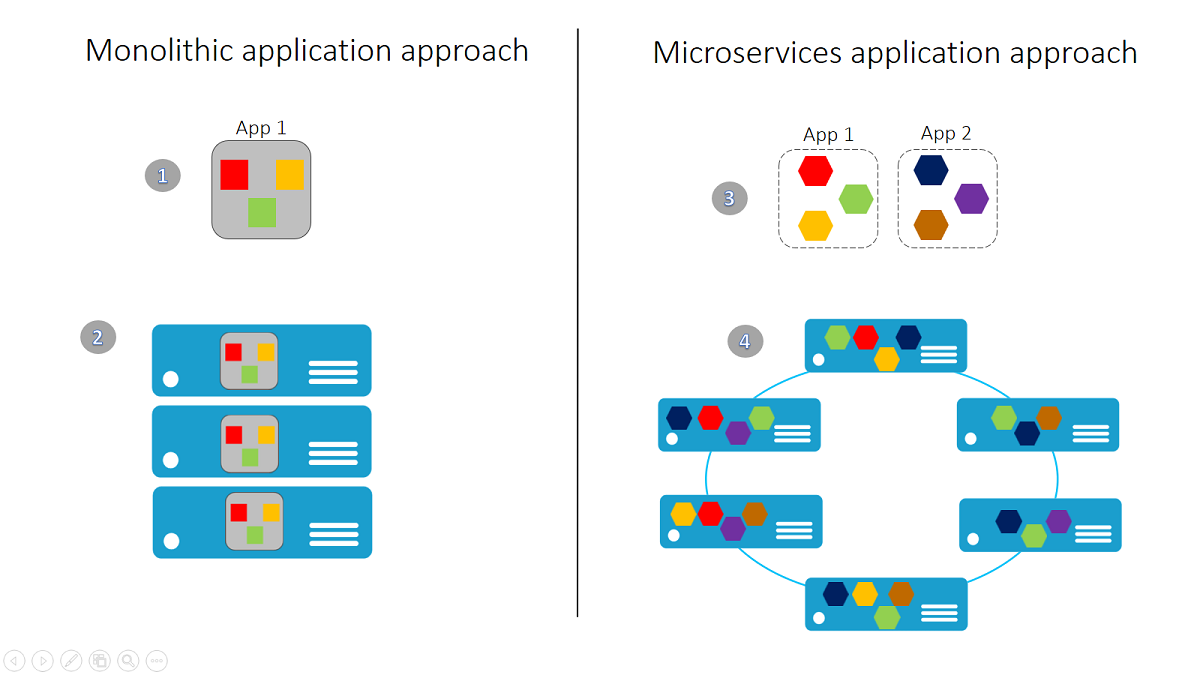
\includegraphics[width=0.9\textwidth]{monolithic_vs_micro}
	\caption{Sie sehen Unterschiede.\cite{nhiem2017mic_moving}}
	\label{fig:trigo_funk}
\end{figure}